\documentclass[10pt,a4paper]{article}
\usepackage[utf8]{inputenc} 
\usepackage[spanish]{babel}
\usepackage{a4wide}
\usepackage{caratula}

\begin{document}

\titulo{Trabajo Práctico}
\subtitulo{SLS: Un simple lenguaje de scripting}

\fecha{\today}

\materia{Teoría de Lenguajes}
\grupo{Los Libres de Contexto}

\integrante{Apellido, Nombre2}{002/01}{email2@dominio.com}
\integrante{Bonomi, Cyntia}{134/03}{cyntiab83@gmail.com}
\integrante{Izcovich, Sabrina}{550/11}{sizcovich@gmail.com}

\maketitle

\tableofcontents

\newpage
\section{Introducción}

\section{Gramática}
EXPRESSIONes regulares de los tokens y transformaciones\\
Tipo de Gramática definida \\


PROGRAM $\rightarrow$ LIST\_SENTENCIES \\

LIST\_SENTENCIES $\rightarrow$ SENTENCE $|$ SENTENCE LIST\_SENTENCIES\\

SENTENCE $\rightarrow$ E; $|$ WHILE $|$ IF\_ELSE $|$ CONDITIONAL $|$ FOR $|$ DO\_WHILE $|$ COMMENT \\

WHILE $\rightarrow$ while (CONDITION) SENTENCE $|$ while (CONDITION) \{ LIST\_SENTENCIES \} \\

IF\_ELSE $\rightarrow$ IF else SENTENCE $|$ IF else \{ LIST\_SENTENCIES \} \\

IF $\rightarrow$ if (CONDITION) SENTENCE $|$ if (CONDITION) \{ LIST\_SENTENCIES \} \\

CONDITIONAL $\rightarrow$ (CONDITION) ? SENTENCE : SENTENCE \\

FOR $\rightarrow$ for(ASIGNACION ;CONDITION; AVANZAR) SENTENCE $|$ (ASIGNACION ;CONDITION; AVANZAR) \{ LIST\_SENTENCIES \} \\

ASIGNACION $\rightarrow$ $\lambda$ $|$ var = EXPRESSION $|$ var[NUM] = EXPRESSION $|$ var[NUM] = EXPRESSION\\

AVANZAR $\rightarrow$ var++ $|$ var$--$ $|$ var -= NUM $|$ var += NUM $|$ $\lambda$ \\

DO\_WHILE $\rightarrow$ do \{ LIST\_SENTENCIES \} while (CONDITION) \\

CONDITION $\rightarrow$ LOGICAL\_CONDITION $|$ CONDITION\_AND $|$ CONDITION\_OR \\

CONDITION\_AND $\rightarrow$ LOGICAL\_CONDITION AND LOGICAL\_CONDITION \\

CONDITION\_OR $\rightarrow$ LOGICAL\_CONDITION OR LOGICAL\_CONDITION \\

LOGICAL\_CONDITION $\rightarrow$ E $>$ E $|$ E $<$ E $|$ E == E $|$ E != E \\

E $\rightarrow$ ASIGNACION $|$ EXPRESSION \\

VALUE $\rightarrow$ string $|$ bool $|$ var $|$ NUM $|$FUNCION $|$ var[NUM] $|$ [LIST\_VALUES] $|$ \{ LIST\_REGISTERS \}\\

LIST\_REGISTERS $\rightarrow$ REGISTER $|$ REGISTER , LIST\_REGISTERS\\

REGISTER $\rightarrow$ cadena:VALUE \\

LIST\_VALUES $\rightarrow$ VALUE $|$ VALUE , LIST\_VALUES \\

EXPRESSION $\rightarrow$  ARITHMETIC\_EXPRESSION $|$ VALUE \\

FUNCTION $\rightarrow$ FUNCTION\_WITH\_RETURN $|$ FUNCTION\_NO\_RETURN \\

FUNCTION\_WITH\_RETURN $\rightarrow$ multiplicacionEscalar(PARAM\_ME) $|$  capitalizar(string) $|$  colineales(var, var) $|$ length(PARAM\_LENGTH) \\

FUNCTION\_NO\_RETURN $\rightarrow$ print(EXPRESSION) \\

PARAM\_ME $\rightarrow$ var, NUM, bool $|$ var, NUM \\

PARAM\_LENGTH $\rightarrow$ var $|$ string \\

LIST\_PARAMETROS $\rightarrow$ EXPRESSION $|$ LIST\_PARAMETROS , EXPRESSION \\

ARITHMETIC\_EXPRESSION $\rightarrow$  + TERM $|$ ARITHMETIC\_EXPRESSION - TERM $|$ TERM \\

TERM $\rightarrow$ TERM $*$ FACTOR $|$ TERM $/$ FACTOR $|$ TERM \% FACTOR $|$ FACTOR \\

FACTOR $\rightarrow$ NUM $|$ var[NUM] \\

NUM $\rightarrow$ decimal $|$ natural


\section{Gramática de Atributos}

PROGRAM $\rightarrow$ LIST\_SENTENCIES \\

\{ LIST\_SENTENCIES.level = 0, PROGRAM.value = LIST\_SENTENCIES.value \} \\ \\


LIST\_SENTENCIES $\rightarrow$ SENTENCE \\

\{ SENTENCE.level = LIST\_SENTENCIES.level, LIST\_SENTENCIES.value = SENTENCE.value \}  \\ \\


LIST\_SENTENCIES $\rightarrow$ SENTENCE  $LIST\_SENTENCIES_{1}$ \\

\{ SENTENCE.level = LIST\_SENTENCIES.level, LIST\_SENTENCIES.value = SENTENCE.value + $LIST\_SENTENCIES_{1}.value$  \} \\  \\


SENTENCE $\rightarrow$  E; \\ 

\{ E.level = SENTENCE.level, SENTENCE.value = E.value \}  \\ \\

SENTENCE $\rightarrow$  WHILE  \\ 

\{ WHILE.level = SENTENCE.level, SENTENCE.value = WHILE.value \}  \\ \\

SENTENCE $\rightarrow$  IF\_ELSE  \\ 

\{ IF\_ELSE.level = SENTENCE.level, SENTENCE.value = IF\_ELSE.value \}  \\ \\

SENTENCE $\rightarrow$  CONDITIONAL  \\ 

\{ CONDITIONAL.level = SENTENCE.level, SENTENCE.value = CONDITIONAL.value \}  \\ \\

SENTENCE $\rightarrow$  FOR \\ 

\{ FOR.level = SENTENCE.level, SENTENCE.value = FOR.value \}  \\ \\

SENTENCE $\rightarrow$  DO\_WHILE \\ 

\{ DO\_WHILE .level = SENTENCE.level, SENTENCE.value = DO\_WHILE .value \}  \\
  
SENTENCE $\rightarrow$  COMMENT \\ 

\{ COMMENT .level = SENTENCE.level, SENTENCE.value = COMMENT .value \}  \\ \\


WHILE $\rightarrow$ while (CONDITION) SENTENCE \\  

\{ SENTENCE.level = WHILE.level + 1, WHILE.value = 'while (' + CONDITION.value + ')' + indentar(SENTENCE.value, SENTENCE.level) \}  \\ \\

WHILE $\rightarrow$ while (CONDITION) \{ LIST\_SENTENCIES \}  \\

\{ LIST\_SENTENCIES.level = WHILE.level + 1, WHILE.value = 'while (' + CONDITION.value + ')\{' + indentar(SENTENCE.value, SENTENCE.level) + '\textbackslash{}n \}' \} \\ \\

IF\_ELSE $\rightarrow$ IF else SENTENCE   \\

\{ SENTENCE.level = IF\_ELSE.level + 1, IF\_ELSE.value = IF.value + 'else ' + indentar(SENTENCE.value, SENTENCE.level) \}  \\ \\

IF\_ELSE $\rightarrow$ IF else \{ LIST\_SENTENCIES \}  \\

\{ LIST\_SENTENCIES.level = IF\_ELSE.level + 1, IF\_ELSE.value = IF.value + 'else {' + indentar(LIST\_SENTENCIES, SENTENCE.level) + '\textbackslash{}n \}' \} \\ \\


IF $\rightarrow$ if (CONDITION) SENTENCE   \\

\{ SENTENCE.level = IF.level + 1, IF.value = 'if (' + CONDITION.value + ') ' + indentar(SENTENCE.value, SENTENCE.level) \}  \\ \\

IF $\rightarrow$ if (CONDITION) \{ LIST\_SENTENCIES \}  \\

\{ LIST\_SENTENCIES.level = IF.level + 1, IF.value = 'if (' + CONDITION.value + '){' + indentar(LIST\_SENTENCIES, SENTENCE.level) + '\textbackslash{}n \}' \} \\ \\


CONDITIONAL $\rightarrow$ (CONDITION) ? $SENTENCE_{1} : SENTENCE_{2}$  \\

\{ $SENTENCE_{1}$.level = CONDITIONAL.level + 1,$SENTENCE_{2}$.level = CONDITIONAL.level + 1 CONDITIONAL.value = '(' + CONDITION.value + ') ?' + $SENTENCE_{1}$.value ': '  + $SENTENCE_{2}$.value \} \\ \\

FOR $\rightarrow$ for(ASSIGNATION ;CONDITION; ADVANCE) SENTENCE  \\

\{ SENTENCE.level = FOR.level + 1, FOR.value = 'for (' + ASSIGNATION.value + ';' +CONDITION.value + AVANZAR.value') ' + indentar(SENTENCE.value, SENTENCE.level) \} \\ \\


FOR $\rightarrow$ (ASSIGNATION ;CONDITION; ADVANCE) \{ LIST\_SENTENCIES \} \\ 

\{ LIST\_SENTENCIES.level = FOR.level + 1, FOR.value = 'for (' + ASSIGNATION.value + ';' +CONDITION.value + ADVANCE.value'){' + indentar(LIST\_SENTENCIES, SENTENCE.level) + '\textbackslash{}n \}' \} \\ \\


ASSIGNATION $\rightarrow$ var = EXPRESSION \\  

\{ ASSIGNATION.value = EXPRESSION.value, setVar(var.name, EXPRESSION.type) \}  \\ \\

ASSIGNATION $\rightarrow$ var[NUM] = EXPRESSION  \\

\{ ASSIGNATION.value = EXPRESSION.value, setVar(var.name, 'array ' + EXPRESSION.type) \}  \\ \\

ASSIGNATION $\rightarrow$ $\lambda$ \\


ADVANCE $\rightarrow$ var++   \\

\{ ADVANCE.value = var.name + ' ++ ' \}  \\ \\


ADVANCE $\rightarrow$ var$--$   \\

\{ ADVANCE.value = var.name + ' -- ' \}  \\ \\


ADVANCE $\rightarrow$ var -= NUM  \\ 

\{ ADVANCE.value = var.name + ' -= ' + NUM.value \}  \\ \\


ADVANCE $\rightarrow$ var += NUM  \\

\{ ADVANCE.value = var.name + ' += ' + NUM.value \}  \\ \\


ADVANCE $\rightarrow$ $\lambda$ \\

DO\_WHILE $\rightarrow$ do \{ LIST\_SENTENCIES \} while (CONDITION) \\

\{ LIST\_SENTENCIES.level = DO\_WHILE.level + 1, DO\_WHILE.value = 'do \{ \textbackslash{}n ' +  indentar(LIST\_SENTENCIES.value, LIST\_SENTENCIES.level)  + '\textbackslash{}n while (' +CONDITION.value +') ' \} \\ \\



CONDITION $\rightarrow$ LOGICAL\_CONDITION   \\
\{ CONDITION.value = LOGICAL\_CONDITION,  CONDITION.type = LOGICAL\_CONDITION.type \}  \\ \\


CONDITION $\rightarrow$ CONDITION\_AND   \\

\{ CONDITION.value = CONDITION\_AND,  CONDITION.type = CONDITION\_AND.type \}  \\ \\

CONDITION $\rightarrow$ CONDITION\_OR \\

\{ CONDITION.value = CONDITION\_OR,  CONDITION.type = CONDITION\_OR.type \}  \\ \\


CONDITION\_AND $\rightarrow$ $LOGICAL\_CONDITION_{1}$ AND $LOGICAL\_CONDITION_{2}$ \\

\{ CONDITION\_AND.value = $LOGICAL\_CONDITION_{1}$.value + ' AND' +  , $LOGICAL\_CONDITION_{2}$,  ONDITION\_AND.type = 'bool' \}  \\ \\


CONDITION\_OR $\rightarrow$ $LOGICAL\_CONDITION_{1}$ OR $LOGICAL\_CONDITION_{2}$ \\


\{ CONDITION\_OR.value = $LOGICAL\_CONDITION_{1}$.value + ' OR' +  , $LOGICAL\_CONDITION_{2}$,  ONDITION\_OR.type = 'bool' \}  \\ \\


\{ LOGICAL\_CONDITION.value = $E_{1}$.value + ' $<$ ' +  , $E_{2}$,  LOGICAL\_CONDITION.type = 'bool' \}  \\ \\


LOGICAL\_CONDITION $\rightarrow$ $E_{1}$ $>$ $E_{2}$   \\

\{LOGICAL\_CONDITION.value = $E_{1}$.value + ' $>$ ' +  , $E_{2}$,  LOGICAL\_CONDITION.type = 'bool' \}  \\ \\

LOGICAL\_CONDITION $\rightarrow$ $E_{1}$ $<$ $E_{2}$   \\

\{LOGICAL\_CONDITION.value = $E_{1}$.value + ' $<$ ' +  , $E_{2}$,  LOGICAL\_CONDITION.type = 'bool' \}  \\ \\


LOGICAL\_CONDITION $\rightarrow$ $E_{1}$ == $E_{2}$   \\

\{LOGICAL\_CONDITION.value = $E_{1}$.value + ' == ' +  , $E_{2}$,  LOGICAL\_CONDITION.type = 'bool' \}  \\ \\

LOGICAL\_CONDITION $\rightarrow$ $E_{1}$ != $E_{2}$ \\

\{LOGICAL\_CONDITION.value = $E_{1}$.value + ' != ' +  , $E_{2}$,  LOGICAL\_CONDITION.type = 'bool' \}  \\ \\


E $\rightarrow$ ASSIGNATION   \\

\{E.value = ASSIGNATION.value  \}  \\ \\

E $\rightarrow$ EXPRESSION \\

\{E.value = EXPRESSION.value  , E.type = EXPRESSION.type \}  \\ \\


VALUE $\rightarrow$ string   \\

\{VALUE.value =  'string' , VALUE.type = 'string' \}  \\ \\


VALUE $\rightarrow$ bool   \\

\{VALUE.value =  'bool' , VALUE.type = 'bool' \}  \\ \\


VALUE $\rightarrow$ var   \\

\{VALUE.value =  var.name , VALUE.type = getType(var.name) \}  \\ \\


VALUE $\rightarrow$ NUM   \\

\{VALUE.value =  NUM.value , VALUE.type = NUM.type \}  \\ \\


VALUE $\rightarrow$ FUNCTION\_WITH\_RETURN \\

\{VALUE.value =  FUNCTION.value , VALUE.type = FUNCTION.type \}  \\ \\

VALUE $\rightarrow$ var[NUM]    \\

\{VALUE.value =  var.value + '[ ' + NUM.value + ']', VALUE.type = 'array ' + NUM.type \}  \\ \\


VALUE $\rightarrow$ [LIST\_VALUES]   \\

\{VALUE.value =  '[ ' + LIST\_VALUES.value + ']', VALUE.type = LIST\_VALUES.type \}  \\ \\

VALUE $\rightarrow$ \{ LIST\_REGISTERS \} \\

\{VALUE.value =  '\{ ' + LIST\_REGISTERS.value + '\}', VALUE.type = 'register' \}  \\ \\



LIST\_REGISTERS $\rightarrow$ ASSIGNATION  \\

\{LIST\_REGISTERS.value =  ASSIGNATION.value  \}  \\ \\

LIST\_REGISTERS $\rightarrow$ ASSIGNATION , $LIST\_REGISTERS{1}$ \\

\{LIST\_REGISTERS.value =  ASSIGNATION.value + ', ' + $LIST\_REGISTERS{1}$  \}  \\ \\



LIST\_VALUES $\rightarrow$ VALUE   \\

\{LIST\_VALUES.value =  VALUE.value, LIST\_VALUES.type = VALUE.type \}  \\ \\

LIST\_VALUES $\rightarrow$ VALUE, $LIST\_VALUES{1}$ \\

\{LIST\_VALUES.value =  VALUE.value + ', ' + $LIST\_VALUES{1}$, LIST\_VALUES.type = actualizarTipoArray(EXPRESSION.type, $LIST\_VALUES{1}$.type ) \}  \\ \\


EXPRESSION $\rightarrow$ ARITHMETIC\_EXPRESSION \\   

\{EXPRESSION.value =  ARITHMETIC\_EXPRESSION.value, EXPRESSION.type = ARITHMETIC\_EXPRESSION.type  \}  \\ \\


EXPRESSION $\rightarrow$ EXPRESSION\_STRING   \\

\{EXPRESSION.value =  EXPRESSION\_STRING.value, EXPRESSION.type = 'string'  \}  \\ \\


EXPRESSION $\rightarrow$ VALUE \\

\{EXPRESSION.value =  VALUE.value, EXPRESSION.type = VALUE.type  \}  \\ \\



FUNCTION $\rightarrow$ FUNCTION\_WITH\_RETURN \\

\{FUNCTION\_WITH\_RETURN.value =  FUNCTION\_WITH\_RETURN.value, FUNCTION.type = FUNCTION\_WITH\_RETURN.type  \}  \\ \\


FUNCTION $\rightarrow$ FUNCTION\_NO\_RETURN \\

\{FUNCTION\_NO\_RETURN.value =  FUNCTION\_NO\_RETURN.value, FUNCTION.type = FUNCTION\_NO\_RETURN.type  \}  \\ \\



FUNCTION\_NO\_RETURN $\rightarrow$ print(EXPRESSION) \\   

\{FUNCTION\_NO\_RETURN.value =  'print (' + EXPRESSION.value + ')', FUNCTION\_NO\_RETURN .type = 'void'  \}  \\ \\


FUNCTION\_WITH\_RETURN $\rightarrow$ multiplicacionEscalar(PARAM\_ME) \\   

\{FUNCTION\_WITH\_RETURN.value =  'multiplicacionEscalar (' + PARAM\_ME.value + ')', FUNCTION\_WITH\_RETURN.type = '??'  \}  \\ \\


FUNCTION\_WITH\_RETURN $\rightarrow$ capitalizar(string)   \\

\{FUNCTION\_WITH\_RETURN.value =  'capitalizar (' + string.value + ')', FUNCTION\_WITH\_RETURN.type = 'string'  \}  \\ \\


FUNCTION\_WITH\_RETURN $\rightarrow$ colineales($var_{1}$, $var_{2}$)   \\

\{CONDITION: (($var_{1}$.type == 'array natural' OR $ var_{1}$.type == 'array decimal') AND
($var_{2}$.type == 'array natural' OR $var_{2}$.type == 'array decimal')), FUNCTION\_WITH\_RETURN.value =  'colineales (' + $var_{1}$.value + ', ' +$var_{2}$')', FUNCTION\_WITH\_RETURN.type = 'bool'  \}  \\ \\


FUNCTION\_WITH\_RETURN $\rightarrow$ length(PARAM\_LENGTH) \\

\{FUNCTION\_WITH\_RETURN.value =  'length (' + PARAM\_LENGTH.value + ')', FUNCTION\_WITH\_RETURN.type = 'natural'  \}  \\ \\



PARAM\_ME $\rightarrow$ var, NUM, bool   \\

PARAM\_ME $\rightarrow$ var, NUM \\

PARAM\_LENGTH $\rightarrow$ var    \\

PARAM\_LENGTH $\rightarrow$ string \\


EXPRESSION\_STRING $\rightarrow$ EXPRESSION\_STRING + string \\  

\{EXPRESSION\_STRING.value =  EXPRESSION\_STRING.value + ' + ' + string.value, EXPRESSION\_STRING.type = 'string') \}  \\ \\


ARITHMETIC\_EXPRESSION $\rightarrow$ ARITHMETIC\_EXPRESSION + TERM   \\

\{ARITHMETIC\_EXPRESSION.value =  ARITHMETIC\_EXPRESSION.value + ' + ' + TERM.value, ARITHMETIC\_EXPRESSION.type = TERM.type) \}  \\ \\


ARITHMETIC\_EXPRESSION $\rightarrow$ ARITHMETIC\_EXPRESSION - TERM  \\

\{ARITHMETIC\_EXPRESSION.value =  ARITHMETIC\_EXPRESSION.value + ' - ' + TERM.value, ARITHMETIC\_EXPRESSION.type = TERM.type) \}  \\ \\


ARITHMETIC\_EXPRESSION $\rightarrow$ TERM \\

\{ARITHMETIC\_EXPRESSION.value = TERM.value, ARITHMETIC\_EXPRESSION.type = TERM.type) \}  \\ \\


TERM $\rightarrow$ $TERM_{1}$ $*$ FACTOR   \\

\{TERM.value = $TERM_{1}$.value + '$*$' + FACTOR.value, TERM.type = ?) \}  \\ \\


TERM $\rightarrow$ $TERM_{1}$ $/$ FACTOR   \\

\{TERM.value = $TERM_{1}$.value + '\%' + FACTOR.value, TERM.type = ?) \}  \\ \\


TERM $\rightarrow$ $TERM_{1}$ \% FACTOR  \\

\{TERM.value = $TERM_{1}$.value + '\%' + FACTOR.value, TERM.type = FACTOR.type) \}  \\ \\


TERM $\rightarrow$ FACTOR \\

\{TERM.value = FACTOR.value, TERM.type = FACTOR.type) \}  \\ \\


FACTOR $\rightarrow$ NUM   \\

\{FACTOR.value = NUM.value, FACTOR.type = NUM.type) \}  \\ \\


FACTOR $\rightarrow$ var[NUM]  \\ 

\{ FACTOR.value = var.name + '[' + NUM.value + ']', FACTOR.type = 'array ' + NUM.type) \}  \\ 
\\

NUM $\rightarrow$ decimal \\

\{ NUM.value = decimal.value, NUM.type = 'decimal') \}  \\ 

NUM $\rightarrow$ natural \\

\{ NUM.value = natural.value, NUM.type = 'natural') \}  \\ 


\section{Ejemplo de la Gramática de Atributos}

\begin{center}
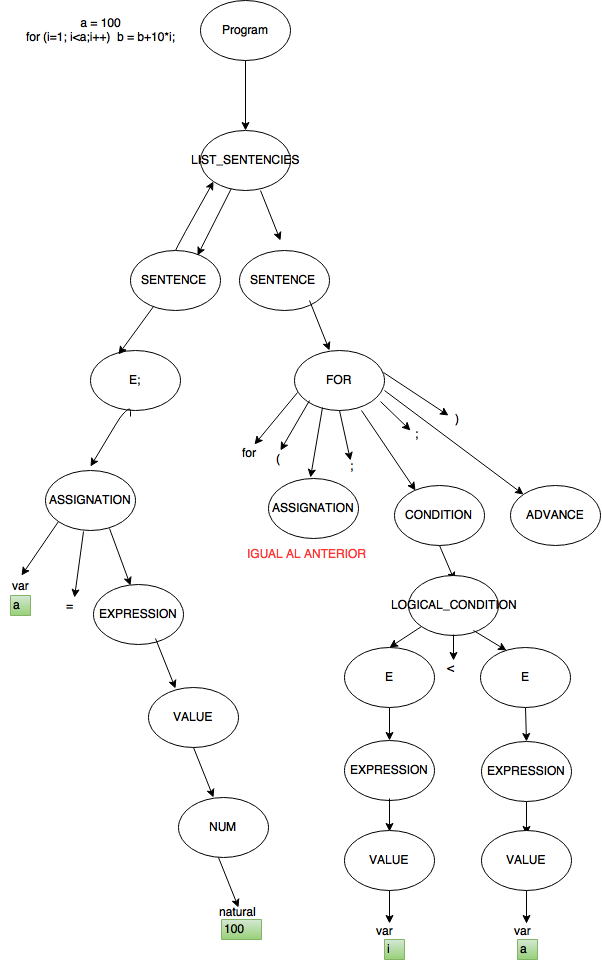
\includegraphics[scale=0.7]{imgs/ejemploGramatica.png}
\end{center}

\section{Descripción}

Asumimos que ASIGNACION $\rightarrow$ VAR = NUM 

Asumimos que los Registers toman únicamente literales de tipos básicos.

Gramática de atributos:

\begin{itemize}
\item \textbf{Value:} string (\textit{sintetizado}) es el código de salida del parser arreglado.
\item \textbf{Level:} int (\textit{heredado}) almacena el nivel de indentación de la producción actual.
\item \textbf{Type:} string (\textit{sintetizado}) representa el tipo de la expresión en cuestión.
\end{itemize}

\section{Compilación y ejecución}

\section{Casos de prueba}

\section{Resultados}

\section{Conclusión}

\section{Referencias}

\end{document}
